\chapter{测试与评估}

\par 本章中我们对我们实现的采用Bundle-K方案的CW-Cache系统进行初步的测试与评估。

\section{实验方法}

\subsection{实验环境设置}

\par 我们在一个6节点的Amazon EC2的集群中搭建Spark、CW-Cache、HDFS组成的平台,其中1台作为Master,其他作为Worker,每个节点是r3.xlarge,各自有4个CPU,30.5 GB内存。我们使用iPerf测得节点之间的网络带宽在740Mbps和1Gbps的范围内。我们在平台上用Spark执行标准测试程序TPC-H提供的SQL查询任务,观察各项指标。所有的查询任务均在Master上进行提交。

\par 实验中所用的测试数据是利用TPC-H标准测试程序工具包生成的规模为$10$的数据,我们利用Spark将其转换为了Parquet格式以进行实验。

\subsection{负载}

\par 我们在第~\ref{chp:cw-cache}章就观察到,执行TPC-H提供的任务便能够造成列的访问热度倾斜,在本评估实验中,我们将TPC-H的22个查询任务依次执行若干次对 系统进行“预热”,目的是让Master在这个过程中对访问的文件片段进行记录,一段时间内收集的信息便可供CW-Cache执行Bundle-K方案进行复制。在这之后,我们会控制应用程序随机启动TPC-H中的任务。

\subsection{对比测试}

\par 在本实验中,我们选择最基本的固定大小分块(Fixed-size Chunking)的方案进行对比,这个方法是很多分布式缓存/存储系统常常采用的,比如HDFS、Windows Azure Storage和Alluxio。在固定大小分块方案中,文件被分成固定大小的文件块,存储在集群中。因为我们的方案是基于Alluxio构建的,因此我们采用原生Alluxio作为CW-Cache方案的对照。

\subsection{衡量指标}

\par 首先是根据SQL查询任务执行的平均时间来计算系统降低延迟的程度,时间的降低我们可以用:
\begin{equation}
    \textstyle \text{Time reduction} = \frac{T_\mathrm{a} - T_\mathrm{cw}}{T_\mathrm{a}} \times 100\%,
    \label{eq:time-reduce}
 \end{equation}
 来计算,其中$T_\mathrm{cw}$ 和 $T_\mathrm{a}$ 表示分别在CW-Cache和原生 Alluxio系统中查询任务执行时间。

\par 此外,我们用\emph{不均衡因子}衡量负载不均衡的程度,它被定义为:
\begin{equation}
    \textstyle \eta = \frac{L_{\mathrm{max}}-L_{\mathrm{avg}}}{L_{\mathrm{avg}}},
    \label{eq:ld-im}
\end{equation}
其中 $L_{\mathrm{max}}$ 和 $L_{\mathrm{avg}}$ 分别是服务器中最大的和平均负载,值更小的$\eta$表明更好的负载均衡。

\section{实验结果}

\subsection{读取延迟}

\begin{figure}[ht]
	\centering
	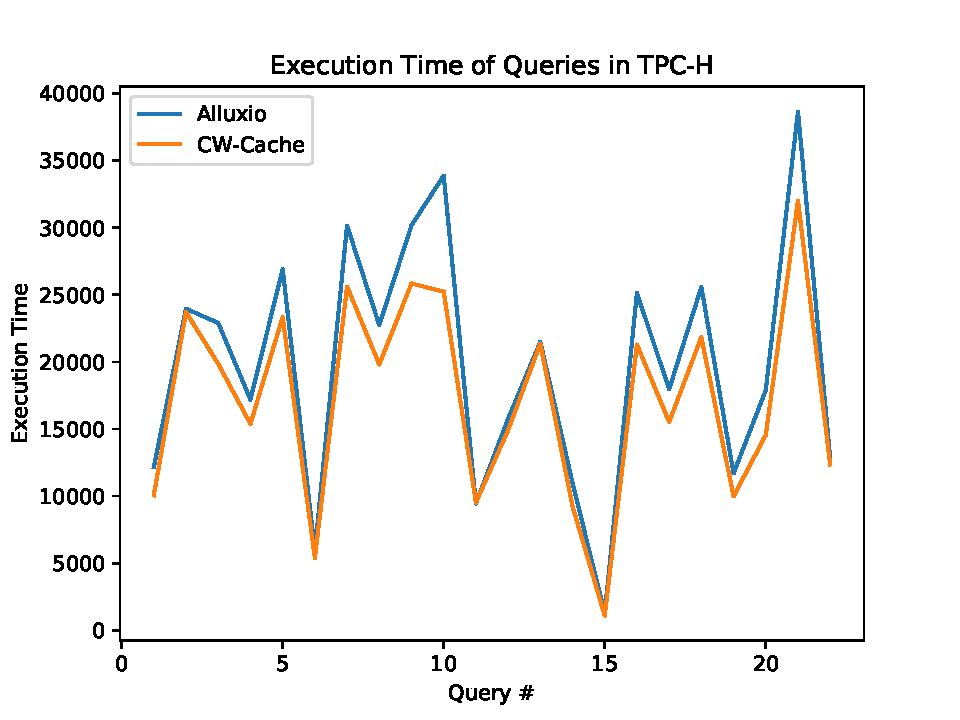
\includegraphics[width=0.70\paperwidth]{img/evaluation/query-execution-time}
	\caption{任务执行时间比较。}
	\label{fig:q-exe}
	%\vspace{-.15in}
\end{figure}

\par 图~\ref{fig:q-exe}是我们得到的两个方案的查询任务的执行时间。由图可以看出,两条曲线的趋势基本一致,我们的CW-Cache比原生Alluxio系统要略好一点,综合这22个SQL任务来看,根据计算可知,平均的$\textstyle \text{Time reduction} = 12\%$,即TPC-H查询任务的执行时间平均降低12\%。多数任务的执行时间降低,但是也有任务执行时间增加,我想可能的原因有:1) 有一部分任务属于计算密集型而不是I/O密集型,其瓶颈在于CPU,我们的方案需要上传访问信息,反而增加Client与Master的通信开销,导致比原生Alluxio稍慢;2) 其次系统是初步实现,还未进行优化,本身性能还为达到令人满意的地步,说明还有很多细节亟待完善。

\subsection{负载}

\begin{figure}[ht]
	\centering
	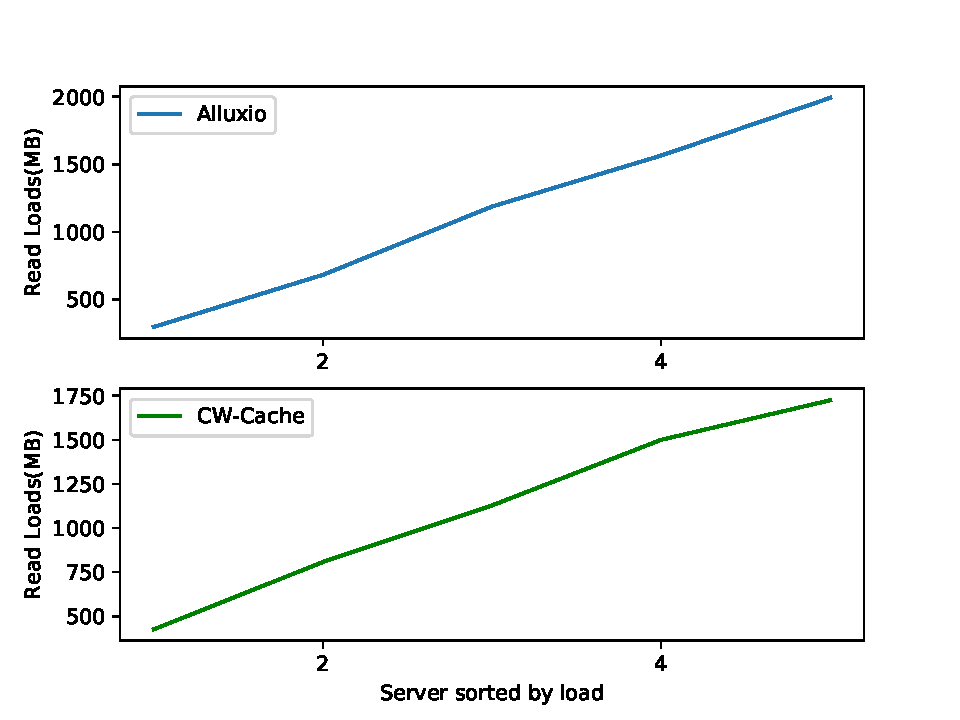
\includegraphics[width=0.70\paperwidth]{img/evaluation/server-load}
	\caption{两种场景下的负载的分布。服务器的负载按照总的数据读取量计算。}
	\label{fig:server-load}
	%\vspace{-.15in}
\end{figure}

\par 图~\ref{fig:server-load}展示了按照服务器负载大小排序后的服务器负载分布。由图可见,CW-Cache优于原生方案。根据\eqref{eq:ld-im}式可以计算出$\eta_a = 0.7398$,$\eta_cw = 0.4442$,那么负载不均衡度减小了$0.26$,一定程度上说明CW-Cache对系统负载均衡有所贡献。

